\section{方法}
\label{sec:method-zh}

\method{} 按照时间顺序处理多镜头单目视频，并将相机、可见人体和场景几何重建到统一世界坐标系中。在每个镜头内部，递归重建器持续更新紧凑的历史表示。在镜头切换处，这些历史仍是建立镜头间空间关系所需的有效参照，却不再适合作为新视觉内容继续传播的递归条件。因此，\method{} 为历史的这两种作用赋予不同的信息生命周期。

如图~\ref{fig:method-zh} 所示，检测到镜头边界后，同一幅新镜头首帧进入两条互补路径。历史条件对齐路径临时读取先前状态以推断镜头间关系，随后即被丢弃；重新初始化重建路径独立开始新镜头，并拥有唯一向后传播的状态。带类型的对齐表示从当前观测与递归历史中组织边界证据。估计得到的镜头关系、基于几何的人物关联和共享变换随后将重新初始化路径的输出提交到已有世界坐标系。该边界操作只使用当前与历史观测，不修改已经输出的帧，也不执行逐视频优化。

\begin{figure*}[t]
  \centering
  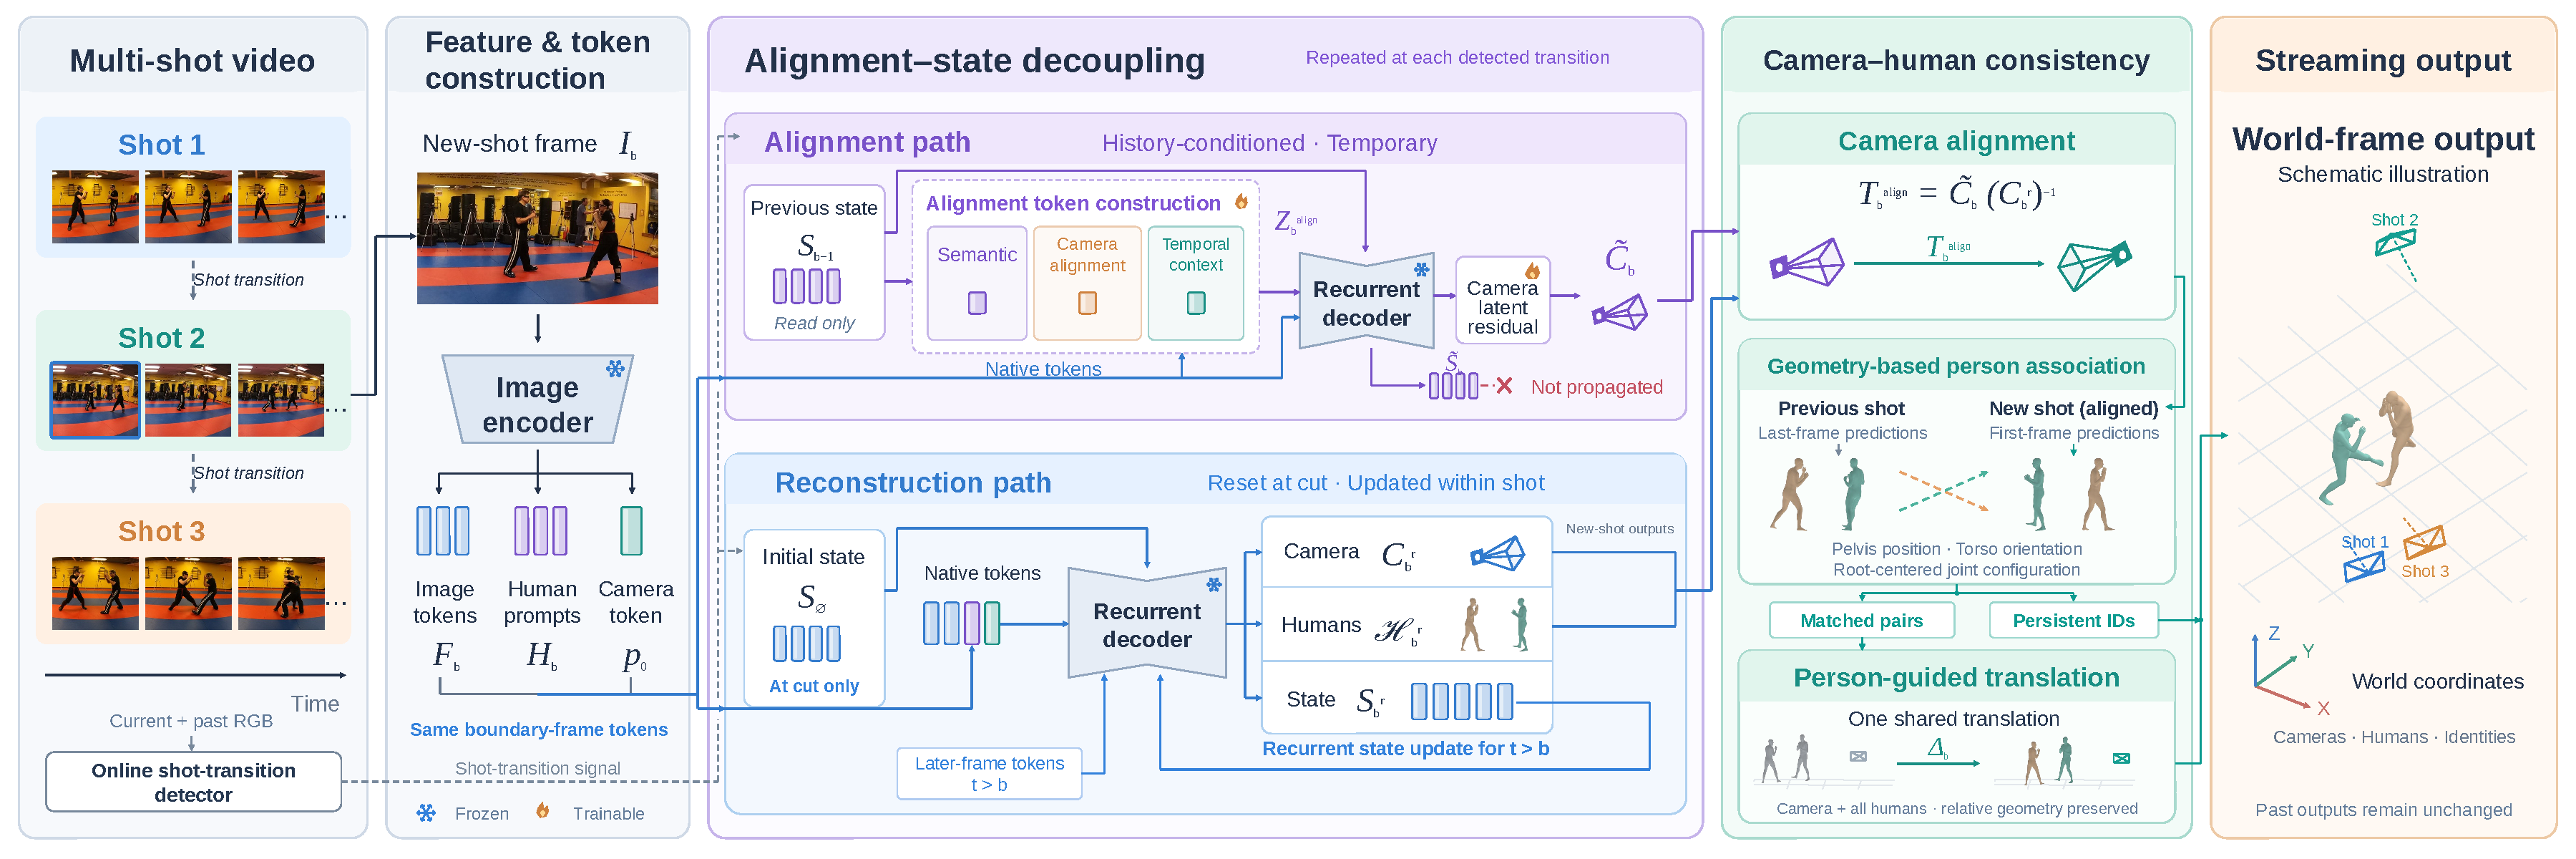
\includegraphics[width=\textwidth]{figures/method.pdf}
  \caption{\method{} 方法概览。历史条件路径临时推断镜头间关系，只有重新初始化路径传播递归状态。基于几何的人物关联延续人物身份，共享变换将新镜头输出置于统一世界坐标系。最右侧面板为示意图。}
  \label{fig:method-zh}
\end{figure*}

\subsection{镜头边界处的递归重建}

给定由连续镜头片段组成的单目视频流 $\{I_t\}_{t=1}^{T}$，\method{} 在时刻 $t$ 仅利用截至当前的观测，在线恢复相机姿态 $C_t$、场景几何 $P_t^w$ 与多个可见人体 $\mathcal H_t$。所有输出均表示在一个统一世界坐标系中：该坐标系由首个镜头初始化，并由所有后续镜头及其相机、人体和场景几何共享，而非外部预先指定的绝对坐标系。将历史观测编码为递归状态 $S_t$，一般的有状态重建过程可以表示为

\begin{equation}
 (y_t,S_t)=f_\theta(I_t,S_{t-1}),\qquad
 y_t=\left(C_t,P_t^w,\{J_t^i,V_t^i,q_t^i\}_{i=1}^{N_t}\right),
 \label{eq:online-map-zh}
\end{equation}

其中，$C_t$ 为 camera-to-world 相机姿态，$J_t^i$、$V_t^i$ 和 $q_t^i$ 分别表示人物 $i$ 的 SMPL-X
~\citep{pavlakos2019smplx}
关节、网格顶点与匿名人物槽位。在实现中，我们使用预训练的 \humanthree{} 递归重建器构造 $f_\theta$，由其提供镜头内的相机、人体与场景预测
~\citep{chen2026human3r}。在连续观测下，$S_{t-1}$ 所承担的空间参照与递归条件两种作用相互兼容；镜头切换则使二者分离。旧状态仍可作为推断新镜头与已有重建之间关系的依据，但其中由上一镜头视角和内容形成的表示，已不再是更新新镜头状态的有效条件。直接传播能够保留空间参照，却可能使这种失配持续影响后续递归；重新初始化能够隔离失配，却同时失去了镜头间的空间关系。

为解决这一冲突，\method{} 在检测到的镜头边界 $b$ 对同一幅新镜头首帧执行两次互补的在线计算：

\begin{equation}
\begin{aligned}
 (\widetilde y_b,\widetilde S_b)&=f_{\theta,\phi}(I_b,S_{b-1}), &
 (y_b^r,S_b^r)&=f_\theta(I_b,S_{\varnothing}),\\
 (y_t^r,S_t^r)&=f_\theta(I_t,S_{t-1}^r), && t>b.
\end{aligned}
\label{eq:boundary-paths-zh}
\end{equation}

历史条件对齐路径读取 $S_{b-1}$，仅用于推断新镜头与已有世界坐标系之间的关系；边界操作完成后，其预测结果和 $\widetilde S_b$ 均被丢弃。重新初始化重建路径从 $S_{\varnothing}$ 出发，并以 $S_b^r$ 作为该镜头后续所有帧唯一的递归状态。因此，镜头间关系估计与新镜头状态传播具有彼此独立的信息路径。

\subsection{历史条件镜头对齐}

历史条件路径需要从新镜头首帧 $I_b$ 与先前状态 $S_{b-1}$ 的交互中估计镜头间空间关系。用于连续重建的递归表示同时包含图像内容、相机运动、人体信息与历史上下文，而镜头边界处的关系推断需要区分这些信息所承担的不同作用。为避免过早将全部证据汇聚成单一校正向量，\method{} 显式构造三种带类型的对齐表示，分别描述语义对应、相机潜变量变化和累积的时间上下文。

令 $c_b$ 表示从当前图像、相机和人体 token 中汇聚的观测证据，$m_{b-1}$ 表示从递归状态与相机记忆中提取的历史证据。三种带类型表示定义为

\begin{equation}
\begin{aligned}
 z_b^{\mathrm{sem}}&=\alpha_b c_b+(1-\alpha_b)m_{b-1}, &
 z_b^{\mathrm{cam}}&=\operatorname{MLP}_{\mathrm{cam}}
 [p_b,p_{b-1},\Delta p_b,m_{b-1}],\\
 z_b^{\mathrm{temp}}&=\operatorname{MLP}_{\mathrm{temp}}
 [\bar z_{b-1},\delta_{b-1},g_{b-1}], &
 Z_b^{\mathrm{align}}&=[z_b^{\mathrm{sem}},z_b^{\mathrm{cam}},z_b^{\mathrm{temp}}].
\end{aligned}
\label{eq:alignment-tokens-zh}
\end{equation}

其中，$\alpha_b$ 自适应调节当前语义证据与历史上下文的贡献；$p_b$ 和 $p_{b-1}$ 为边界两侧的相机 token，$\Delta p_b=p_b-p_{b-1}$ 表示其潜变量变化；$\bar z_{b-1}$、$\delta_{b-1}$ 和 $g_{b-1}$ 分别表示此前的对齐摘要、相机潜变量残差及其门控强度。三种表示并非相互独立的重建模块，而是对异质边界信息进行分类型组织，使不同证据在进入解码器时保持来源可辨。

\noindent
\begin{minipage}[t]{0.57\textwidth}
\vspace{0pt}
加入类型嵌入后，$Z_b^{\mathrm{align}}$ 被插入原生相机 token 之后，并与图像、相机和人体表示共同通过冻结的递归主干。解码后的边界表示产生门控的相机与人体潜变量残差。前者在原有相机预测头输出临时相机 $\widetilde C_b$ 之前更新相机表示；后者将人物平移约束纳入同一边界推断过程。所有带类型表示与潜变量更新仅存在于对齐路径中，不会写入新镜头随后传播的状态。汇聚与残差分支的完整定义见英文补充材料。

\smallskip
我们同时使用镜头切换与连续四帧序列训练对齐表示。镜头切换样本由两个相机的 $A(t),A(t+1),B(t+2),B(t+3)$ 构成，用于监督视角切换前后的变化；连续样本由同一相机的连续四帧构成，用于维持连续输入下的原有重建行为。
\end{minipage}\hfill
\begin{minipage}[t]{0.39\textwidth}
  \vspace{0pt}
  \centering
  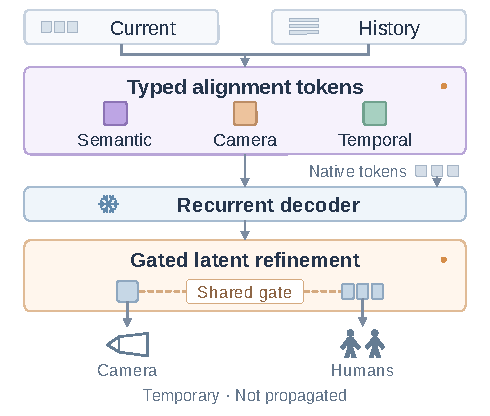
\includegraphics[width=0.94\linewidth]{figures/alignment_module.pdf}
  \captionof{figure}{\textbf{历史条件镜头对齐。}带类型表示组织当前与历史证据；门控潜变量更新仅存在于临时路径。}
  \label{fig:alignment-module-zh}
\end{minipage}

\medskip
对齐训练目标联合监督相机平移、相机旋转、人体平移、残差门控以及校正有效性：

\begin{equation}
 \mathcal L_{\mathrm{align}}=\mathcal L_t+5\mathcal L_R+10\mathcal L_h
 +0.05(\mathcal L_g+\mathcal L_{\mathrm{imp}})
 +10^{-5}(\mathcal R_{\mathrm{cam}}+\mathcal R_{\mathrm{human}}),
 \label{eq:alignment-objective-zh}
\end{equation}

其中，$\mathcal L_t$ 与 $\mathcal L_h$ 为相机和人体平移的 Smooth-L1 损失，$\mathcal L_R$ 为四元数测地距离。令 $e$ 和 $e^{\mathrm{raw}}$ 分别表示归一化后的校正相机误差与未校正误差，则门控与有效性约束为
$\mathcal L_g=\operatorname{BCE}(g,\operatorname{clip}(e^{\mathrm{raw}},0,1))$ 和
$\mathcal L_{\mathrm{imp}}=[e-e^{\mathrm{raw}}]_+$，其余两项用于正则化相机与人体潜变量更新。镜头切换改变的是历史信息与当前观测之间的关系，而不是镜头内的重建目标。因此，我们仅优化带类型表示、相机与人体潜变量残差分支，以及预测头中的低秩适配参数
~\citep{hu2022lora}；图像编码器、递归主干、基础预测头和 Multi-HMR 组件
~\citep{baradel2024multihmr}
均保持冻结。

\subsection{跨镜头空间与身份一致性}

重新初始化路径隔离了不兼容历史对新镜头递归过程的影响，但其预测位于独立初始化的局部坐标系中。跨镜头关系只有在不重新引入先前递归状态的情况下作用于这些预测，才能将其提交到统一世界坐标系。为此，\method{} 仅保留边界时刻推断出的相机关系并将其作用于重新初始化路径的输出；临时对齐状态没有进入后续递归的通路。由于两条路径处理同一幅图像，其相对相机姿态反映了历史条件所确定的空间关系。令 $C_b^r$ 表示重新初始化路径预测的 camera-to-world 姿态，$\widetilde C_b$ 表示已经表达在累计统一世界坐标系中的临时对齐路径相机姿态，则新镜头局部坐标系的初始映射为

\begin{equation}
 T_b^{\mathrm{align}}=\widetilde C_b(C_b^r)^{-1}.
 \label{eq:inter-shot-alignment-zh}
\end{equation}

该变换满足 $T_b^{\mathrm{align}}C_b^r=\widetilde C_b$，因此可以将重新初始化路径的相机和人体预测映射到已有坐标系。对于后续镜头切换，$\widetilde C_b$ 已包含此前累计的镜头间变换。需要强调的是，$T_b^{\mathrm{align}}$ 来自边界处当前观测与递归历史的特征交互，而不是在两个镜头完成重建后对其输出执行事后配准。

相机关系本身不能确定人物对应。完成初始空间映射后，\method{} 使用预测的人体根节点位置、躯干朝向和去除根节点平移后的关节结构建立一对一关联。对于线索 $a\in\{\mathrm{root},\mathrm{torso},\mathrm{joint}\}$，我们分别归一化其成对代价矩阵，并构造联合代价：

\begin{equation}
 \widehat d_{ij}^{\,a}=
 \frac{d_{ij}^{\,a}}
 {\max\!\left(\operatorname{median}_{u,v}d_{uv}^{\,a},\epsilon\right)},
 \qquad
 d_{ij}=\widehat d_{ij}^{\,\mathrm{root}}
       +\widehat d_{ij}^{\,\mathrm{torso}}
       +\widehat d_{ij}^{\,\mathrm{joint}}.
 \label{eq:association-cost-zh}
\end{equation}

其中，根节点项为欧氏距离，躯干项为角距离，关节项为去除根节点平移后对应关节欧氏距离的均值。通过 Hungarian assignment
~\citep{munkres1957assignment}
得到匹配集合 $\mathcal M_b$。匹配不使用身份标注、外部相机标定或后续帧。匹配人物继承上一镜头的匿名身份，未匹配的新镜头人物槽位获得新的身份。该置换只在新镜头首帧建立一次，后续帧保留重新初始化递归所维持的原生人物槽位。

初始相机映射确定新镜头的朝向及其与已有坐标系的主要关系，匹配人物则为剩余的共享平移提供直接约束。令 $r_{b-1}^i$ 表示上一镜头末帧中人物 $i$ 的预测骨盆中心，$\bar r_b^j$ 表示完成初始映射后新镜头首帧中人物 $j$ 的骨盆中心，我们估计

\begin{equation}
 \Delta_b=\lambda\underset{(i,j)\in\mathcal M_b}{\operatorname{median}}
 (r_{b-1}^i-\bar r_b^j),\qquad \lambda=0.5,
 \label{eq:shared-translation-zh}
\end{equation}

其中，中位数沿三个空间坐标分别计算，固定的 $\lambda$ 在所有数据集上保持不变。当边界处没有有效匹配时，不施加该平移，仅保留相机关系给出的初始映射。令
$T_b^\Delta=\begin{bmatrix}I_3&\Delta_b\\\mathbf 0^\top&1\end{bmatrix}$ 且
$T_b=T_b^\Delta T_b^{\mathrm{align}}$，则对于 $t\geq b$，最终提交的输出为

\begin{equation}
\begin{aligned}
 C'_t&=T_bC_t^r, &
 J_t^{\prime i}&=T_bJ_t^{r,i}, &
 V_t^{\prime i}&=T_bV_t^{r,i},\\
 P_t^{\prime,w}&=C'_tP_t^{r,c}=T_bP_t^{r,w}, &
 q_t^{\prime i}&=\pi_b(q_t^{r,i}), &
 S'_t&=S_t^r.
\end{aligned}
\label{eq:shared-world-transform-zh}
\end{equation}

其中，$\pi_b$ 表示边界处得到的身份映射，三维点均使用齐次坐标。相机局部场景点图 $P_t^{r,c}$ 保持不变，其世界坐标表示由变换后的相机姿态一致地确定。同一个世界变换作用于相机和全部人体，从而保持二者的相对几何；保留 $S_t^r$ 则确保只有重新初始化状态进入未来的重建过程。变换被缓存，并在后续帧被依次处理时作用于其输出。整个过程不访问后续帧、不执行序列级优化，也不修改已经输出的历史结果。
